% !TeX program = xelatex
% !TeX encoding = UTF-8
% !TeX TXS-program:compile = txs:///xelatex | txs:///xelatex
\documentclass[aspectratio=169, table, 12pt]{beamer}
% Preamble bersama seluruh slide mata kuliah ini.
% Dipanggil dari slides/sessionXX/sessionXX.tex tepat sesudah baris
% \documentclass[aspectratio=169, table, 12pt]{beamer}
% Paket tambahan yang hanya dibutuhkan satu sesi ditulis di berkas sesi itu.

\usepackage{colortbl}
\usepackage{xcolor}
\usepackage{listings}
\usepackage{tabularx}
\usepackage{booktabs}
\usepackage{tikz}
\usepackage{pgfplots}
\usepackage{fontspec}
\usepackage[english,bahasai]{babel}
\pgfplotsset{compat=1.18}
\usetikzlibrary{arrows.meta, positioning, calc, fit, shapes.geometric,
  shapes.multipart, backgrounds, matrix, chains, trees}

\makeatletter
\def\input@path{{../theme/}}
\makeatother
\graphicspath{{../theme/}{../../figures/}}
% Stub symlink Windows memakai tema cadangan sampai aset institusi tersedia.
\IfFileExists{../theme/beamerthemePradita.sty}{%
  \usetheme{Pradita}
}{%
  \usetheme{Madrid}
  \setmainfont{TeX Gyre Heros}
  \setsansfont{TeX Gyre Heros}
  \setbeamertemplate{navigation symbols}{}
}

\definecolor{praditagreen}{RGB}{37, 113, 71}
\setbeamercolor{structure}{fg=praditagreen}
\setbeamercolor{palette primary}{bg=praditagreen,fg=white}
\setbeamercolor{palette secondary}{bg=praditagreen!80!black,fg=white}
\setbeamercolor{palette tertiary}{bg=praditagreen!60!black,fg=white}
\setbeamerfont{frametitle}{size=\large}
\setbeamertemplate{caption}[numbered]

% Ukuran header mengikuti teks agar judul panjang tidak menabrak logo.
\setbeamercolor{frametitle}{bg=white,fg=black}
\setbeamertemplate{frametitle}{%
  \begin{beamercolorbox}[wd=\paperwidth,sep=0.2cm]{frametitle}
    \begin{minipage}[c]{0.77\paperwidth}
      \raggedright\fontsize{16}{18}\selectfont\bfseries\insertframetitle
      \ifx\insertframesubtitle\empty\else
        \par\small\mdseries\insertframesubtitle
      \fi
    \end{minipage}\hfill
    \begin{minipage}[c]{0.15\paperwidth}
      \IfFileExists{../theme/classFiles/logo_universitas.png}{%
        
\includegraphics[width=\linewidth]{../theme/classFiles/logo_universitas.png}%
      }{}
    \end{minipage}
  \end{beamercolorbox}
}
\setbeamertemplate{footline}{%
  \ifnum\value{framenumber}>1
    \begin{beamercolorbox}[wd=\paperwidth,ht=0.35cm,dp=0.15cm,
      leftskip=0.3cm,rightskip=0.3cm]{palette primary}
      \footnotesize\bfseries\insertframenumber/\inserttotalframenumber
      \hfill IT40513
    \end{beamercolorbox}
  \fi
}
\DeclareRobustCommand{\berkas}[1]{\path{#1}}

% Tema membuat garis tabel berwarna putih. Dikembalikan agar tabel terbaca.
\arrayrulecolor{black}
\setlength{\arrayrulewidth}{0.5pt}

\lstdefinelanguage{yaml}{
  basicstyle=\ttfamily\scriptsize,
  keywordstyle=\color{blue}\bfseries,
  commentstyle=\color{gray}\itshape,
  stringstyle=\color{red},
  showstringspaces=false,
  breaklines=true,
  frame=lines,
  numbers=none,
  backgroundcolor=\color{lightgray!10},
  tabsize=2,
  morecomment=[l]{\#}
}

\lstdefinelanguage{json}{
  basicstyle=\ttfamily\scriptsize,
  stringstyle=\color{red},
  commentstyle=\color{gray},
  breaklines=true,
  showstringspaces=false,
  tabsize=2,
  numbers=none,
  frame=lines,
  backgroundcolor=\color{lightgray!10},
  string=[s]{"}{"}
}

\lstdefinelanguage{bash}{
  keywords={},
  basicstyle=\ttfamily\scriptsize,
  ndkeywords={docker, kubectl, helm, curl, git, terraform},
  ndkeywordstyle=\color{purple}\bfseries,
  sensitive=true,
  commentstyle=\color{gray},
  numbers=none,
  breaklines=true,
  frame=lines,
  backgroundcolor=\color{lightgray!10},
  tabsize=2,
  comment=[l]{\#},
  showstringspaces=false
}

\lstdefinelanguage{http}{
  keywords={GET, POST, PUT, PATCH, DELETE, HEAD, OPTIONS, HTTP},
  basicstyle=\ttfamily\scriptsize,
  keywordstyle=\color{blue}\bfseries,
  sensitive=true,
  numbers=none,
  breaklines=true,
  frame=lines,
  backgroundcolor=\color{lightgray!10},
  tabsize=2,
  showstringspaces=false
}

\subtitle{IT40513 · Enterprise Architecture \& Digital Blueprint}
\author{\textbf{Alfa Yohannis}}


% Sampul membatasi judul di panel putih tema rujukan Pradita.
\setbeamertemplate{title page}{%
  \begin{tikzpicture}[remember picture,overlay]
    \node[anchor=north west,inner sep=0pt,text width=8.8cm]
      at ([xshift=1cm,yshift=-3.15cm]current page.north west) {%
        {\small\insertsubtitle\par}\vspace{0.25cm}
        \resizebox{8.8cm}{!}{\begin{minipage}{12cm}
          \raggedright\color{praditagreen}\bfseries\inserttitle
        \end{minipage}}
      };
    \node[anchor=south west,inner sep=0pt]
      at ([xshift=1cm,yshift=1.65cm]current page.south west)
      {\small\insertdate};
    \node[anchor=west,inner sep=0pt,text=white]
      at ([xshift=0.8cm,yshift=0.75cm]current page.south west)
      {\small\insertauthor};
  \end{tikzpicture}
}


% Batasi kedua dimensi gambar agar diagram bersama tetap berada pada slide.
\newsavebox{\eafigbox}
\newcommand{\eadiagram}[1]{%
  \sbox{\eafigbox}{\resizebox{0.94\textwidth}{!}{\input{#1}}}%
  \ifdim\dimexpr\ht\eafigbox+\dp\eafigbox\relax>0.64\textheight
    \resizebox{!}{0.64\textheight}{\usebox{\eafigbox}}%
  \else
    \usebox{\eafigbox}%
  \fi
}

\title{\Huge Strategi, Model Operasi,\\ \vspace{10pt} dan Visi Arsitektur}
\date{Pertemuan 03}
\begin{document}
\begin{frame}
  \titlepage
\end{frame}

\begin{frame}
  \frametitle{Isi Pertemuan}
  \vspace{14pt}
  \begin{columns}[t]
    \column{0.5\textwidth}
    {\small\tableofcontents[sections={1-3}]}

    \column{0.5\textwidth}
    {\small\tableofcontents[sections={4-6}]}
  \end{columns}
\end{frame}

\begin{frame}{\hfill}
  \centering
  \Huge{\textbf{Strategi sudah disahkan.\\Mengapa tiap proyek\\menafsirkannya sendiri?}}
\end{frame}

\section{Tujuan dan Konteks}

\begin{frame}{\hfill}
  \centering
  \Huge{\textbf{Tujuan dan Konteks}}
\end{frame}

\begin{frame}{{\Large Tujuan Pembelajaran}}
  \vspace{10pt}
  \begin{itemize}
    \item Menurunkan pemicu, tujuan, dan \textit{outcome} organisasi menjadi kebutuhan arsitektur
          yang dapat ditelusuri.
    \item Menentukan model operasi organisasi berdasarkan tingkat integrasi dan standardisasi
          proses bisnisnya.
    \item Merumuskan visi arsitektur dan prinsip arsitektur lengkap dengan alasan dan
          implikasinya.
  \end{itemize}
\end{frame}

\begin{frame}{{\Large Satu Strategi, Tiga Usulan Proyek}}
  \vspace{10pt}
  \begin{itemize}
    \item Strategi 2026 sampai 2030: ``Satu Pasien, Satu Rekam Medis''.
    \item Belum terjawab: sistem mana berubah, siapa memiliki identitas pasien.
    \item Tim Medikara+ ingin menambah nomor akun pasien baru.
    \item Satu rumah sakit ingin membeli aplikasi antrean sendiri.
    \item Vendor menawarkan pemindahan seluruh aplikasi ke \textit{cloud} pada 2027.
  \end{itemize}
  \vspace{6pt}
  {\small Ketiganya mengaku mendukung strategi. Dua di antaranya menambah salinan data.}
\end{frame}

\begin{frame}{{\Large Diagram Konsep Bab 3}}
  \centering
  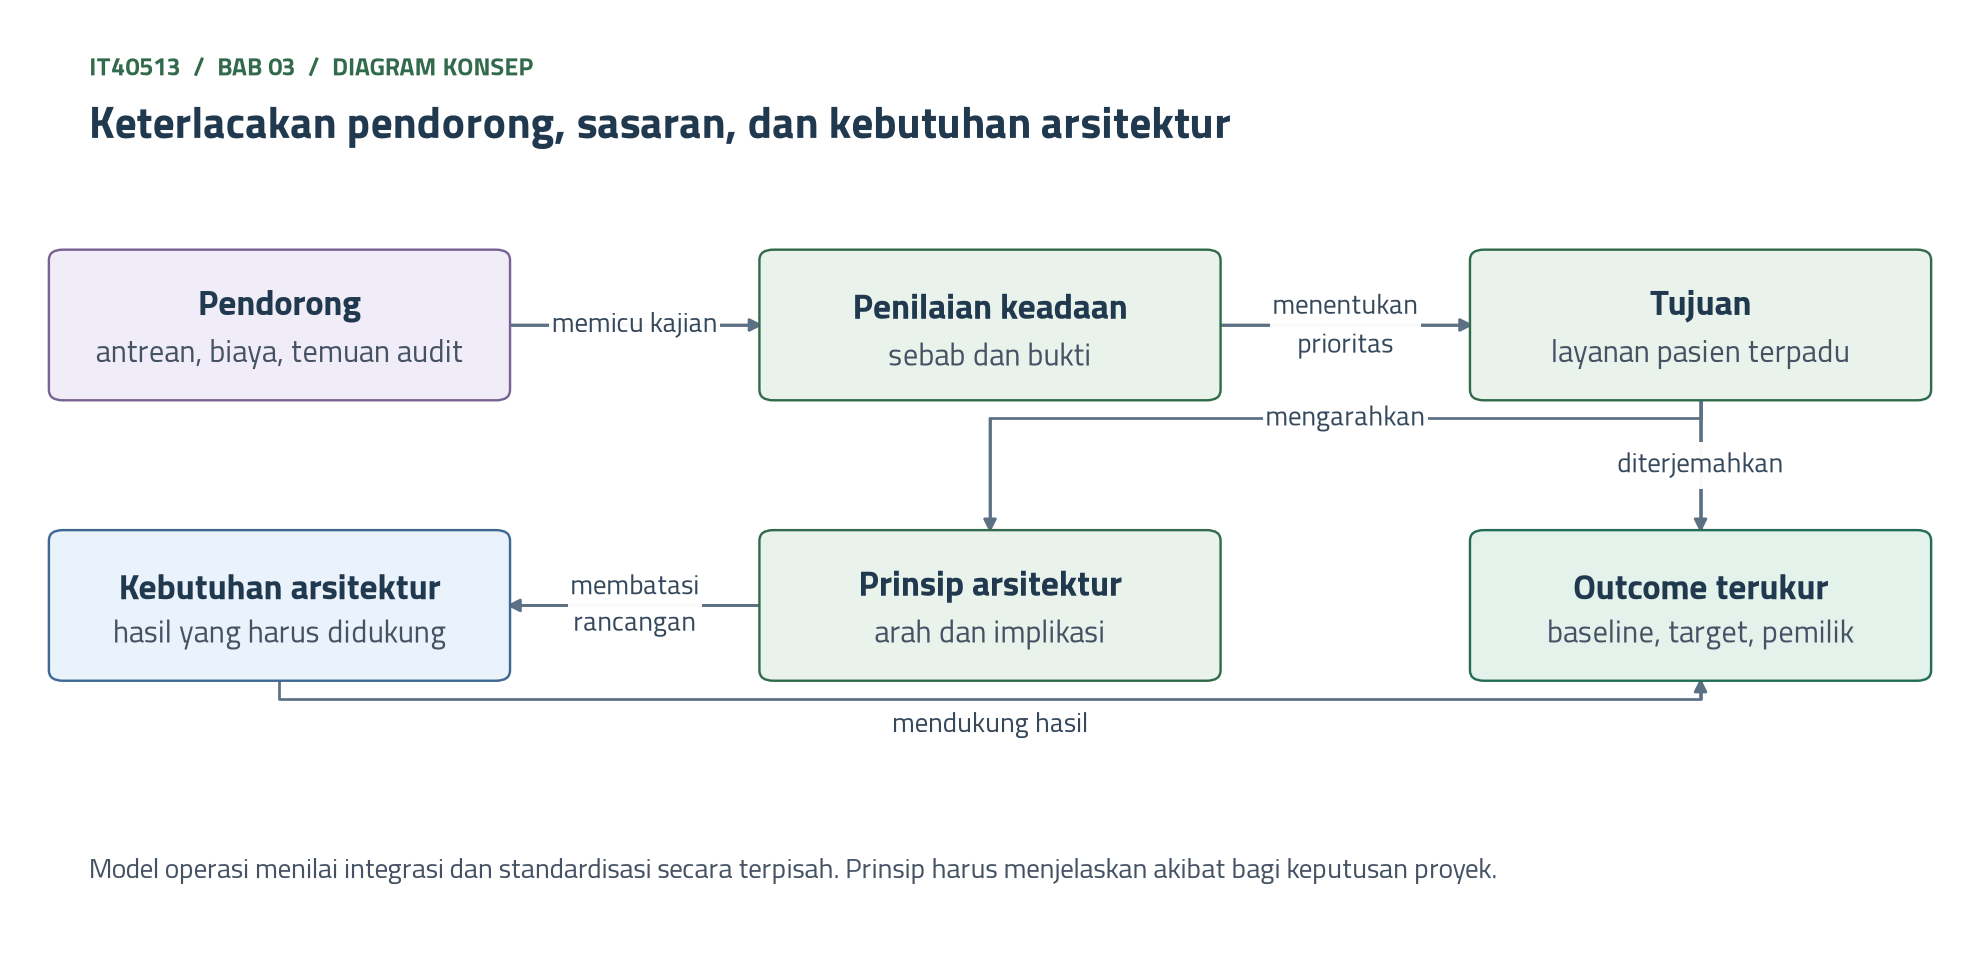
\includegraphics[width=0.96\textwidth,height=0.77\textheight,keepaspectratio]{../../figures/ch03-diagram-konsep.png}
  \label{fig:session03-ilustrasi-bab}
\end{frame}

\section{Rantai Motivasi}

\begin{frame}{\hfill}
  \centering
  \Huge{\textbf{Rantai Motivasi}}
\end{frame}

\begin{frame}{{\Large Enam Elemen Motivasi}}
  \footnotesize
  \begin{tabularx}{\textwidth}{>{\raggedright\arraybackslash}p{2.1cm}
      >{\raggedright\arraybackslash}p{3.9cm} >{\raggedright\arraybackslash}X}
    \hline
    \textbf{Elemen} & \textbf{Pertanyaan} & \textbf{Contoh Medikara} \\
    \hline
    \textit{Driver} & Apa yang menekan organisasi? & Antrean rawat jalan panjang \\
    \hline
    \textit{Assessment} & Seberapa parah, apa penyebabnya? & Tunggu rata-rata 96 menit; jadwal disalin manual \\
    \hline
    \textit{Goal} & Ke mana organisasi bergerak? & Pasien dilayani tepat waktu di mana pun \\
    \hline
    \textit{Outcome} & Bagaimana tahu sudah tercapai? & 96 menjadi 60 menit, Desember 2028 \\
    \hline
    Prinsip & Aturan apa yang memandu pilihan? & Satu sumber kebenaran untuk data pasien \\
    \hline
    \textit{Requirement} & Apa yang harus dipenuhi sistem? & Jadwal dibaca dari SIMRS, jeda paling lama 5 menit \\
    \hline
  \end{tabularx}

  \vspace{6pt}
  {\small Analogi: mobil baru tidak melancarkan ruas jalan yang macet.}
\end{frame}

\begin{frame}{{\Large Rantai dari Pemicu sampai Kebutuhan}}
  \centering
  \eadiagram{../../figures/ch03-rantai-motivasi.tex}
\end{frame}

\begin{frame}{{\Large Lima Isian pada Setiap Outcome}}
  \footnotesize
  \begin{tabularx}{\textwidth}{>{\raggedright\arraybackslash}p{2cm}
      >{\raggedright\arraybackslash}X >{\raggedright\arraybackslash}X}
    \hline
    \textbf{Isian} & \textbf{Antrean rawat jalan} & \textbf{Identitas ganda} \\
    \hline
    Ukuran & Rata-rata menit pendaftaran sampai diperiksa & Nomor milik orang yang punya nomor di rumah sakit lain \\
    \hline
    Kondisi awal & 96 menit & Diukur pada C2, sampel 10.000 nomor \\
    \hline
    Target & 60 menit & Paling banyak 2\% \\
    \hline
    Tenggat & Desember 2028 & Desember 2028 \\
    \hline
    Pemilik & Direktur Pelayanan & Direktur Pelayanan \\
    \hline
  \end{tabularx}

  \vspace{6pt}
  {\small Turun 36 menit atau 37,5 persen. Bab 6 mengukur identitas ganda: 11,4 persen.}
\end{frame}

\begin{frame}{{\Large Hasil Proyek dan Hasil Bisnis}}
  \vspace{10pt}
  \begin{itemize}
    \item Hasil proyek: barang yang diserahkan, misalnya fitur jadwal selesai.
    \item Hasil bisnis: perubahan yang dialami pasien atau organisasi.
    \item Misalkan fitur selesai tepat waktu, tetapi tunggu baru 96 menjadi 91 menit.
    \item Itu baru sekitar 14 persen dari penurunan 36 menit yang ditargetkan.
    \item Penyebabnya cara kerja: formulir kertas dan jadwal yang masih disalin manual.
  \end{itemize}
\end{frame}

\begin{frame}{{\Large Keterlacakan Dua Arah}}
  \vspace{10pt}
  \begin{itemize}
    \item Ke atas menjawab mengapa, ke bawah menjawab bagaimana.
    \item Satu kebutuhan boleh punya banyak induk, asalkan tiap hubungan punya alasan.
    \item Cacat pertama: kebutuhan tanpa induk, misalnya ``seluruh aplikasi ke \textit{cloud}
          pada 2027''.
    \item Cacat kedua: \textit{goal} tanpa \textit{outcome}, misalnya ``paling inovatif''.
    \item Misalkan rantai C1 berisi 15 elemen, 1 dari 3 \textit{requirement} tanpa induk.
  \end{itemize}
\end{frame}

\begin{frame}{{\Large Kasus Medikara: Menguji Tiga Usulan}}
  \vspace{10pt}
  \begin{itemize}
    \item Pertanyaan ujinya satu: elemen mana yang menjadi induknya?
    \item Nomor akun baru: tanpa induk, bertentangan dengan satu sumber kebenaran.
    \item Aplikasi antrean: tampak mendukung 60 menit, tetapi menambah salinan jadwal keenam.
    \item \textit{Cloud} 2027: searah strategi, tetapi belum punya \textit{outcome} terukur.
    \item Pemicu keempat, biaya integrasi tinggi, menjadi bahan Aktivitas.
  \end{itemize}
\end{frame}

\section{Model Operasi}

\begin{frame}{\hfill}
  \centering
  \Huge{\textbf{Model Operasi}}
\end{frame}

\begin{frame}{{\Large Dua Dimensi, Empat Model}}
  \vspace{10pt}
  \begin{itemize}
    \item Model operasi: tingkat integrasi dan standardisasi proses bisnis yang dibutuhkan.
    \item Integrasi: unit berbagi data atau transaksi agar layanan berjalan.
    \item Standardisasi: unit mengikuti cara kerja yang serupa.
    \item Empat model: diversifikasi, koordinasi, replikasi, unifikasi.
    \item Tidak ada kuadran yang otomatis paling baik.
  \end{itemize}
  \vspace{6pt}
  {\small Analogi: kedai bermenu sama tidak berbagi pesanan; bengkel rujukan berbagi riwayat.}
\end{frame}

\begin{frame}{{\Large Empat Kuadran dan Posisi Medikara}}
  \centering
  \eadiagram{../../figures/ch03-model-operasi.tex}
\end{frame}

\begin{frame}{{\Large Empat Model Operasi}}
  \footnotesize
  \begin{tabularx}{\textwidth}{>{\raggedright\arraybackslash}p{1.9cm}
      >{\raggedright\arraybackslash}p{1.6cm} >{\raggedright\arraybackslash}X
      >{\raggedright\arraybackslash}X}
    \hline
    \textbf{Model} & \textbf{Integrasi, standardisasi} & \textbf{Ciri} & \textbf{Ditonjolkan di \textit{core diagram}} \\
    \hline
    Diversifikasi & Rendah, rendah & Unit mandiri, pelanggan berbeda & Teknologi dan layanan bersama \\
    \hline
    Koordinasi & Tinggi, rendah & Pelanggan sama, transaksi saling terlihat & Data bersama, penghubung, pelanggan \\
    \hline
    Replikasi & Rendah, tinggi & Unit serupa, cara kerja sama & Proses utama, otomasi \\
    \hline
    Unifikasi & Tinggi, tinggi & Satu bisnis, proses dan data global & Proses, data, penghubung, otomasi, pelanggan \\
    \hline
  \end{tabularx}
\end{frame}

\begin{frame}{{\Large Core Diagram Arah Medikara}}
  \centering
  \eadiagram{../../figures/ch03-core-diagram.tex}
\end{frame}

\begin{frame}{{\Large Kasus Medikara: Model per Lingkup}}
  \vspace{10pt}
  \begin{itemize}
    \item Layanan pasien saat ini: diversifikasi, akibat akuisisi, bukan pilihan.
    \item Rujukan: misalkan 2.400 pasien per bulan, identitas dan riwayat harus terbaca.
    \item Arah layanan pasien: paling tidak koordinasi; seberapa jauh diputuskan di Bab 8.
    \item Keuangan: 36 fasilitas, satu bagan akun, sudah unifikasi.
    \item Konsekuensi: pemilik definisi data bersama dan mekanisme keputusan.
  \end{itemize}
\end{frame}

\section{Fase Awal dan Prinsip}

\begin{frame}{\hfill}
  \centering
  \Huge{\textbf{Fase Awal dan Prinsip}}
\end{frame}

\begin{frame}{{\Large Artefak Fase Preliminary dan Fase A}}
  \footnotesize
  \begin{tabularx}{\textwidth}{>{\raggedright\arraybackslash}p{3.6cm}
      >{\raggedright\arraybackslash}X >{\raggedright\arraybackslash}X}
    \hline
    \textbf{Artefak} & \textbf{Pertanyaan keputusan} & \textbf{Bukti persetujuan} \\
    \hline
    \textit{Request for Architecture Work} & Mengapa diperlukan sekarang? & Sponsor, pemicu, batas anggaran \\
    \hline
    Prinsip arsitektur & Aturan apa yang memandu pilihan? & Disahkan direksi \\
    \hline
    Visi arsitektur & Arah dan nilai apa yang diwujudkan? & Hasil, lingkup, risiko disepakati \\
    \hline
    \textit{Statement of Architecture Work} & Siapa mengerjakan apa dan kapan? & Ditandatangani sponsor dan pemilik arsitektur \\
    \hline
  \end{tabularx}

  \vspace{6pt}
  {\small Analogi: renovasi gedung. Batas dan penanggung jawab disepakati sebelum gambar rinci.}
\end{frame}

\begin{frame}{{\Large Alur Sampai Persetujuan}}
  \centering
  \eadiagram{../../figures/ch03-alur-visi.tex}
\end{frame}

\begin{frame}{{\Large Skenario Bisnis dan Kesiapan}}
  \vspace{10pt}
  \begin{itemize}
    \item Skenario menyebut pelaku, pemicu, kondisi awal, kejadian normal, kegagalan, hasil.
    \item Misalkan pasien dari Depok dirujuk ke Jakarta; 2 dari 5 pemeriksaan diulang.
    \item Kesiapan menilai visi, kebutuhan, pendanaan, sponsor, tata kelola, kapasitas.
    \item Misalkan 2 dari 6 faktor mendapat skor 1: tata kelola data dan kapasitas TI.
    \item Keduanya masuk visi sebagai risiko beserta tindakannya.
  \end{itemize}
\end{frame}

\begin{frame}{{\Large Prinsip Arsitektur: Empat Bagian}}
  \vspace{10pt}
  \begin{itemize}
    \item Nama: mudah disebut dalam rapat.
    \item Pernyataan: aturan pilihan yang dipakai menilai rancangan.
    \item Alasan: nilai bagi organisasi dan tautan ke tujuan.
    \item Implikasi: pekerjaan, biaya, dan wewenang yang harus ditanggung.
  \end{itemize}
  \vspace{6pt}
  {\small Analogi: ``Pinjaman hanya untuk kebutuhan produktif atau darurat'' menjawab banyak
  permohonan yang belum pernah ada.}
\end{frame}

\begin{frame}{{\Large Dari Kartu Prinsip ke Dua Opsi}}
  \centering
  \eadiagram{../../figures/ch03-anatomi-prinsip.tex}

  \vspace{6pt}
  {\small Bila kedua opsi sama-sama lolos, pernyataan prinsip perlu dipertajam.}
\end{frame}

\begin{frame}{{\Large Prinsip, Slogan, dan Standar}}
  \footnotesize
  \begin{tabularx}{\textwidth}{>{\raggedright\arraybackslash}p{1.8cm}
      >{\raggedright\arraybackslash}X >{\raggedright\arraybackslash}X
      >{\raggedright\arraybackslash}X}
    \hline
    \textbf{Jenis} & \textbf{Contoh} & \textbf{Sifat} & \textbf{Ditinjau saat} \\
    \hline
    Slogan & ``Utamakan pasien'' & Harapan tanpa konsekuensi & Tidak dapat ditinjau \\
    \hline
    Prinsip & ``Akses berdasarkan kebutuhan'' & Aturan pilihan, ada implikasi & Strategi berubah \\
    \hline
    Standar & ``Gunakan versi produk X'' & Pilihan teknis, mudah berubah & Versi produk berubah \\
    \hline
  \end{tabularx}

  \vspace{8pt}
  \small Lima ciri menurut TOGAF: mudah dipahami, kokoh, lengkap, konsisten, stabil.

  \vspace{4pt}
  Uji utama: dua opsi nyata harus dinilai berbeda. Misalkan 3 dari 9 usulan gagal uji ini.
\end{frame}

\begin{frame}{{\Large Konflik, Dispensasi, dan Hak Memutuskan}}
  \vspace{10pt}
  \begin{itemize}
    \item Berbagi data dan pembatasan akses dapat berkonflik; urutan pertimbangan ditulis.
    \item Dispensasi punya pemilik, masa berlaku, alasan, dan rencana kembali.
    \item Misalkan dispensasi 6 bulan untuk \textit{spreadsheet} antrean satu rumah sakit.
    \item Weill dan Ross: prinsip TI satu dari lima keputusan TI utama.
    \item Tim menyusun, kepala TI dan pemilik layanan menguji, direksi mengesahkan.
  \end{itemize}
\end{frame}

\begin{frame}{{\Large Kasus Medikara: Enam Prinsip C1}}
  \footnotesize
  \begin{tabularx}{\textwidth}{>{\raggedright\arraybackslash}p{5.3cm}
      >{\raggedright\arraybackslash}X}
    \hline
    \textbf{Nama} & \textbf{Implikasi utama} \\
    \hline
    PA1 Satu sumber kebenaran untuk data pasien & Pemilik ditunjuk; salinan diberi tanda waktu \\
    \hline
    PA2 Akses berdasarkan kebutuhan & Peran ditinjau tiap tiga bulan \\
    \hline
    PA3 Identitas pasien milik organisasi & 36 fasilitas memetakan nomor lokal \\
    \hline
    PA4 Perubahan berangkat dari kebutuhan & Usulan menyebut induknya \\
    \hline
    PA5 Pertukaran lewat antarmuka baku & \textit{Point-to-point} baru butuh dispensasi \\
    \hline
    PA6 Keleluasaan lokal di luar inti & Daftar inti yang wajib sama disahkan \\
    \hline
  \end{tabularx}
\end{frame}

\section{Visi untuk Direksi}

\begin{frame}{\hfill}
  \centering
  \Huge{\textbf{Visi untuk Direksi}}
\end{frame}

\begin{frame}{{\Large Delapan Bagian Visi Arsitektur}}
  \footnotesize
  \begin{tabularx}{\textwidth}{>{\raggedright\arraybackslash}p{3.6cm}
      >{\raggedright\arraybackslash}X}
    \hline
    \textbf{Bagian} & \textbf{Pertanyaan direksi} \\
    \hline
    Masalah dan pemicu & Mengapa perlu bertindak sekarang? \\
    \hline
    Visi dan hasil & Apa yang berubah bagi pasien dan organisasi? \\
    \hline
    Arah model operasi & Pilihan apa yang disetujui, dan apa yang dikorbankan? \\
    \hline
    Prinsip & Aturan apa yang mengikat proyek berikutnya? \\
    \hline
    Lingkup dan batas & Apa yang tidak akan dikerjakan? \\
    \hline
    Nilai dan ukuran & Apa nilainya, dan seberapa yakin angkanya? \\
    \hline
    Risiko dan kesiapan & Apa yang dapat menggagalkan, dan siapa yang menangani? \\
    \hline
    Keputusan yang diminta & Apa yang harus diputuskan hari ini? \\
    \hline
  \end{tabularx}

  \vspace{6pt}
  {\small Dua sampai tiga halaman. Analogi: usulan rute perjalanan, bukan daftar merek kendaraan.}
\end{frame}

\begin{frame}{{\Large Nilai Ditulis Menurut Jenisnya}}
  \vspace{10pt}
  \begin{itemize}
    \item Tiga jenis nilai: manfaat layanan, penghindaran kerugian, penghematan anggaran.
    \item Misalkan 200.000 kunjungan rawat jalan per tahun di satu rumah sakit.
    \item $200.000 \times 36$ menit $= 7.200.000$ menit, atau 120.000 jam per tahun.
    \item Angka itu manfaat layanan, bukan kas masuk.
    \item Janji vendor ``hemat 30 persen'' ditandai hipotesis sampai kondisi awal diukur.
  \end{itemize}
\end{frame}

\begin{frame}{{\Large Kasus Medikara: Ringkasan Visi C1}}
  \small
  \textbf{Visi.} Pada 2030, setiap pasien punya satu identitas dan satu rekam medis yang dapat
  dibuka dengan aman oleh tenaga kesehatan yang berhak di fasilitas mana pun.

  \vspace{4pt}
  \textbf{Keputusan yang diminta.}
  \begin{itemize}
    \item Koordinasi sebagai batas minimum arah layanan pasien.
    \item Enam prinsip disahkan.
    \item Direktur Pelayanan menjadi pemilik data identitas pasien.
    \item Pengukuran kondisi awal pada C2 disetujui.
  \end{itemize}
  \vspace{4pt}
  \textbf{Belum diputuskan.} Produk SIMRS, lokasi penyimpanan, dan urutan paket kerja.
\end{frame}

\section{Aktivitas dan Latihan}

\begin{frame}{\hfill}
  \centering
  \Huge{\textbf{Aktivitas dan Latihan}}
\end{frame}

\begin{frame}{{\Large Aktivitas: Menyusun Visi Arsitektur}}
  \vspace{6pt}
  \begin{itemize}
    \item Analis bisnis: telaah strategi, wawancara, \textit{goal} dan \textit{outcome}.
    \item Analis teknologi: pemicu dari sistem dan kendala teknis.
    \item Pemodel: keterlacakan rantai dan \textit{core diagram}.
    \item Koordinator: visi dua sampai tiga halaman, selaras dengan tiga mata kuliah lain.
    \item Seluruh tim: model operasi serta lima sampai delapan prinsip.
  \end{itemize}
  \vspace{4pt}
  {\small Berkas: \berkas{sources/chapter03/README.md}. Tim Medikara merantai biaya integrasi.}
\end{frame}

\begin{frame}{{\Large Luaran C1 dan Kriteria Penilaian}}
  \footnotesize
  \begin{tabularx}{\textwidth}{>{\raggedright\arraybackslash}p{4.6cm}r
      >{\raggedright\arraybackslash}X}
    \hline
    \textbf{Kriteria} & \textbf{Bobot} & \textbf{Tanda terpenuhi} \\
    \hline
    Keterlacakan & 30\% & \textit{Requirement} tertelusur sampai \textit{driver} \\
    \hline
    Kejelasan hasil & 25\% & \textit{Outcome} punya lima isian \\
    \hline
    Alasan pilihan dan konsekuensi & 25\% & Ada bukti dan hal yang dikorbankan \\
    \hline
    Konsistensi bukti dan lingkup & 20\% & Fakta dan pengandaian terpisah \\
    \hline
  \end{tabularx}

  \vspace{8pt}
  \small Luaran: visi arsitektur dengan rantai motivasi, model operasi, prinsip, dan
  \textit{core diagram}. Luaran ini menutup tonggak C1.

  \vspace{4pt}
  Data organisasi nyata wajib seizin organisasi dan dianonimkan.
\end{frame}

\begin{frame}{{\Large Ringkasan}}
  \vspace{10pt}
  \begin{itemize}
    \item Rantai motivasi menjaga setiap kebutuhan punya alasan bisnis.
    \item \textit{Outcome} punya ukuran, kondisi awal, target, tenggat, dan pemilik.
    \item Model operasi dinilai per lingkup, dengan bukti integrasi dan standardisasi terpisah.
    \item Prinsip yang baik membuat dua opsi nyata dinilai berbeda.
    \item Rancangan dimulai dari arah yang disepakati, sebelum produk dipilih.
  \end{itemize}
\end{frame}

\begin{frame}{{\Large Latihan}}
  \vspace{10pt}
  \begin{itemize}
    \item Latihan 1: turunkan ``Satu Pasien, Satu Rekam Medis'' menjadi satu \textit{goal}, dua
          \textit{outcome} terukur, dan satu \textit{requirement}.
    \item Latihan 2: 12 apotek berproses sama, pelanggan jarang berpindah cabang. Model operasi
          mana, dan apa akibatnya bagi aplikasi dan data?
    \item Latihan 3: kritik ``Semua sistem harus memakai teknologi terbaru'', lalu tulis ulang
          lengkap dengan alasan dan implikasi.
  \end{itemize}
\end{frame}

\begin{frame}{{\Large Bacaan dan Berkas Pendukung}}
  \vspace{10pt}
  \begin{itemize}
    \item \href{https://www.opengroup.org/togaf}{The TOGAF Standard, 10th Edition (2025 Update)}
    \item \href{https://publications.opengroup.org/standards/archimate/c226}{ArchiMate 3.2 Specification}
    \item Ross, Weill, dan Robertson (2006). \textit{Enterprise Architecture as Strategy}.
    \item Greefhorst dan Proper (2011). \textit{Architecture Principles}.
    \item \berkas{sources/chapter03/README.md}
  \end{itemize}
\end{frame}

\end{document}
